% Chapter Template

\chapter{Convolutional Neural Networks} % Main chapter title
\label{Chapter3}
\def \teoria {Figures/teoria}
\def \path	 {Figures/C3}
%--------------------------------------------------------------------%	SECTION 1
%--------------------------------------------------------------------
%% da completare
In this chapter an overview on the convolutional neural networks is presented. Being a wide subject, an in-depth theoretical discussion would account only for the content of this thesis, which is why the topics are introduced with the aim of having a smattering to understand the applications developed in the following chapters. 

\section{Introduction}

The convolutional neural networks, to which we will refer from now on with the abbreviation \emph{CNN} are an evolution of the regular \emph{deep artificial networks} characterized by a particular architecture extremely advantageous for visual tasks which made them, over the years, very effective and popular. They were inspired by the biological research of Hubel and Wiesel who, by studying cats' brains, had discovered that their visual cortex contained a complex organized cell structure. The latter were sensitive to small local portions of the visual field, called \emph{receptive fields}. Receptive fields acts as perfect local filters to understand the local correlation of the objects in an image. As these systems are the most efficient in nature for image comprehension, researchers have thus attempted to simulate them. 

%--------------------------------------------------------------------
%	SECTION 2
%--------------------------------------------------------------------

\section{Architecture overview}
CNNs are deep neural networks consisting of several layers that act as extractors of the features and a fully-connected network at the end, which acts as a classifier, as shown in the figure \ref{fig:cnn1}. 

\begin{figure}[h!]
 \centering
 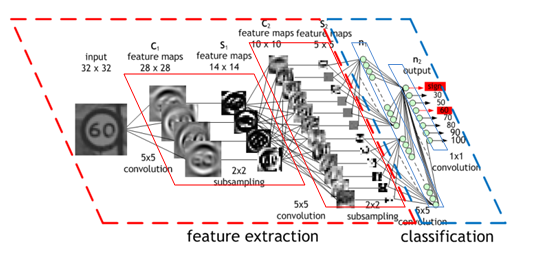
\includegraphics[width=1.0\textwidth]{\path/CNN-expl.png} 
 \caption{Architecture of a CNN that classifies road signs: the image highlights the division between the layers that act as a feature extractor and the final classifier}
 \label{fig:cnn1}
\end{figure}

The stages that perform feature extraction are called \emph{convolutional} layers, they are the fundamental building blocks of CNNs to which they give the name. The latter are usually followed by a non-linear \emph{activation function} and a \emph{pooling} layer. A classical example of a CNN is represented in \ref{fig:cnn2}.

\begin{figure}[h!]
 \centering
 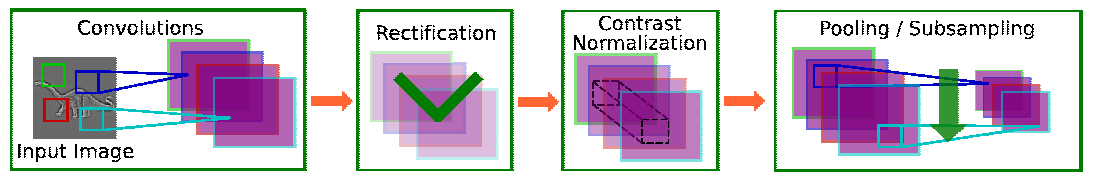
\includegraphics[width=1.0\textwidth]{\path/CNN-features.png} 
 \caption{Typical layers of a convolutional neural networks}
 \label{fig:cnn2}
\end{figure}


Every type of layer has a different goal that fall into four main categories: (i) feature extraction; (ii) non-linear activations; (iii) parameters reduction and skimming. Namely, while convolutional layers search for features of image features, pooling layers squeeze the input to reduce the otherwise huge number of parameters of a CNN; non-linear units serves to enhance the strongest features and weaken the less important ones. i.e. those that have stimulated the neurons less (it is said that they act as "squashing").

From figure \ref{fig:cnn1}, we can also note that to each input image correspond, in the various layers, different groups of output images, which are called \emph{feature maps}. Feature maps are the result of the convolution operation carried out through a filter bank (also called kernels), which are nothing more than matrices with useful values to search for certain characteristics in the images.
\\
Finally, after the convolutional steps, the feature maps are "flattened" in vectors and entrusted to a "classical" neural network (like a multi-layer perceptron, support vector machines, ...) that performs the final classification. 

The number of convolution stages is arbitrary. Initially, when CNN became famous thanks to Y. LeCun, who trained a CNN called \emph{"LeNet5"} to recognize digits \parencite{lenet}, this number ranged from 2 to 4. In 2012, Alex Krizhevsky et al \parencite{imagenet2012} trained a CNN which consists of 5 convolution layers, 60 million parameters and 650 thousand neurons. They obtained the lowest error rate by far on the ImageNet ILSVRC-2010 dataset, containing 1.2 million images divided into 1000 categories.
\\
Since then, things have evolved with terrific speed, and the same ImageNet challenge of 2015 was won by a model with 152 layers \parencite{resnet}. 

As CNN models grow deeper and wider, the need for compression strategies have become more and more important. 

\subsection{Convolutional layer} 
To fully understand what actually happens inside a CNN, it is necessary to introduce the concept of convolution between matrices, and to understand how this is important to process a digital image through a filter.

\subsection{Spatial 2D convolution}
Originally, convolution is defined in functional analysis as a mathematical operator on two functions $f$ and $g$ that produces a third function, that measures the integral of the pointwise multiplication of $f$ and $g$ translated by a certain amount $\tau$. 

Formally: 
\begin{equation}
    (f*g)(t):=\int_{-\infty}^{\infty} f(\tau)g(t-\tau) d\tau= \int_{-\infty}^{\infty} f(t-\tau)g(\tau) d\tau
\end{equation}

% In the context of signal processing, convolution is fundamental as it models the impulsive response of a system with respect to an input signal.

A digital image can be considered as a matrix $A$ of $I\times J$ real or discrete values. Each matrix value is called \emph{pixel} and its indices are also called coordinates: each pixel $A(i, j)$ represents the intensity at the position indicated by the indices. 
\\
A "filter" or "kernel"  is a small matrix used to apply a certain transformation to an image e.g., blurring, sharpening, edge detection and more. The transformation is applied by means of a convolution operation between the input image and the filter. Thus, images and filters can be modeled as 2D signals. Moreover, images and filters are finite supports and hence the integral can be approximated by a finite summation. Therefore, the  convolution is discrete and can be defined as: 
\begin{equation}
\label{eq:2Dconvolution}
    Y(i,j) = X* h = \sum_{u=-k}^{k} \sum_{v=-k}^{k}x(i,j) h(i-u,j-v)
\end{equation}

Each pixel of $ Y(i, j)$ is the result of a weighed sum the sub-region that is centered in the pixel indicated by the coordinates $i,j$. Intuitively, a 2D spatial convolution consists in sliding a window of size $2k+1 \times 2k+1$ on the image $X$ and compute the operation indicated in \ref{eq:2Dconvolution} for each pixel centered on the window. 


An example of convolution is represented in figure \ref{fig:convolution}. 

\begin{figure}[h!]
 \centering
 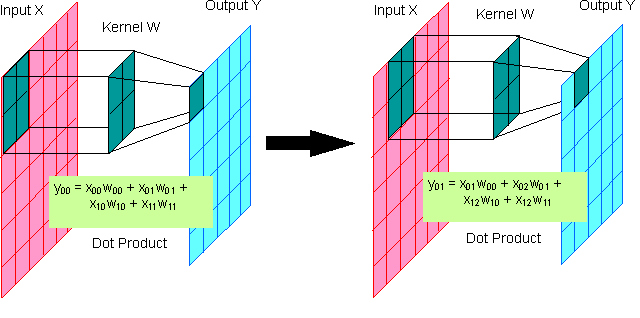
\includegraphics[width=0.7\textwidth]{\path/convolution.png} 
 \caption{Convolution with a kernel: first two steps}
 \label{fig:convolution}
\end{figure}


In the convolutional layers, a convolution operation is performed between the input image(s) and an arbitrary number $K$ of filters. These filters have particular values, called   \emph{weights},  best suited to enhance certain characteristics of the inputs. 
\\
The basic idea is that initially these weights are chosen according to some random distribution and then they are improved at each iteration by the \emph{backpropagation} algorithm \parencite{backprop}. 
\newline 
In this way, the network trains its filters to extract the most important features of the training set examples; thus by changing training set the values of the filters will be different. For example, the weights of a network trained on images of vertical posts will be different from one trained on images of cars; in the first case the values will be calibrated to recognize long vertical orientations, while in the second to recognize more complex rectangular shapes. Therefore, in CNNs the actual learning accumulates in the convolutional filter banks. Artificial \emph{neurons} in these networks, must be understood as the individual filters.


There are several so called \emph{"hyperparameters"} that have to be set manually in the convolutional layers:

\begin{enumerate} 
     \item the filter size $F$: also called \emph{receptive field}. Each filter searches for a specific feature in a local area of the image, thus the filter size is the receptive field of the single neuron. They typically are of size $3 \times3$, $5 \times 5$ or $7\times7$.
     
     \item The $K$ number of filters: for each layer, this value defines the depth of the convolution operation output. In fact, by placing the feature maps on top of each other, you get a cube in which each "slice" is the result of the operation between the input image and the corresponding filter. The depth of this cube depends precisely on the number of filters.
     
     \item The \emph{"stride"} $S$: defines of how many pixels the convolution filter slides at each step. For instance, if the horizontal stride is set to 2, the filter will move towards the x-axis of 2 pixels at a time, skipping one column each time and thus producing a smaller output.
     
     \item The \emph{"padding"} $P$: defines the measure with which we want to add pad to the input with zeros to preserve the same size on the output. In general, when stride $S=1$, a value of $P=(F-1)/2$ ensures that the output will be of the same size as the input.
\end{enumerate}

\\

When processing images with CNNs, inputs are typically three-dimensional, characterized by the height $H_1$, the amplitude $W_1$ and the number of input channels $D_1$. Knowing the parameters specified above, we can calculate the size of the output of a convolution layer: 
\begin{align*}
H_2 &=(H_1-F+2P)/S+1\\
W_2 &=(H_1-F+2P)/S+1\\
D_2 &= K
\end{align*}

In this regard, we can observe the "volume of neurons" of the first convolution layer in figure \ref{fig:depth}. Each neuron is said to be \emph{locally connected}, i.e. spatially connected only to one local region of the input but to the whole depth. 


Note that there are five neurons along the depth and each one looks at the same region of the input but with different weights. In fact, each filter map of the volume of neurons, has its own set of weights. The former is particularly useful when searching for different features on the same region of the input. This is best showed in figure \ref{fig:weights}. 
\newline 

On the other side, each neuron of the same filter map share the same set of weights. This important property is called \emph{parameter sharing} and has the advantage of reducing the number of parameters by a significant factor, saving a lot of computation and memory. This is also depicted in \ref{fig:weights}.  

\begin{figure}[h!]
 \centering
 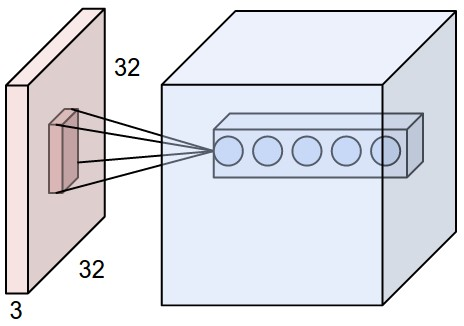
\includegraphics[width=0.4\textwidth]{\path/depthcol.jpeg} 
 \caption{Each neuron is connected to only 1 local region of the input but in total depth (i.e. the three color channels in thi). The depth of the output is given by the K number of filters, in this case 5}
 \label{fig:depth}
\end{figure}

 Convolutional layers show interesting properties. Firstly, they are translation-invariant: in fact, if a feature in an image is translated, it will be translated by the same amount in the feature map, but will still be detected since each neuron in that map share the same weights. Also, feature maps will remain unchanged elsewhere. This property is the basis to its robustness with respect to translations and distortions of the input image. 
 
 secondly, by lining up several convolution layers, a CNN is able to have a more "abtract" (i.e. semantic) understanding of the image. The first convolution layer deals with extracting features directly from the raw pixels of the image and it stores them in the feature maps. This output then becomes the input of a subsequent convolution level, which will do a second extraction of the characteristics, combining the information of the previous layer. From this multi-level abstraction comes a greater understanding of the image features.
 
 \subsection{Convolution over volumes}

 
 \subsection{Convolution complexity}
 \label{subsec:cnn-complexity}
 In order to understand the complexity of a convolutional layer in terms of multiplications-addictions (mult-adds) is better to break down what happens exactly in a convolutional forward pass with an example. 
 Let $K$ be a squared kernel of size $3 \times 3$, $U$ an input feature map of size $12 \times 12 \times 16$ where $"12"$ is the spatial dimension of the input and $"16"$ its channel depth, and $V$ an output feature map of depth $32$.
 
 Each of the 16 channels of $U$ is traversed by 32 $3\times3$ kernels resulting in 512 $(16x32)$ feature maps. Next, they will be merged in 1 feature map out of every input channel by adding them up. That means there will be 32 sums and thus the output size will be of 32, as said above. 
 \newline 
 
 More generally, given a squared kernel of size $d \times d$, an input feature map of size $H \times W \times S$ where $H$ and $W$ are the spatial dimension of the input and $S$ its depth, and an output feature map of depth $T$, the number of multiplications-additions operation of a \emph{single} convolutional layer amounts to: 
 \begin{equation}
    S\cdot d \cdot d \cdot T 
 \end{equation}
 
 It is important to remind that this calculations come from the fact that \emph{all} input maps are convolved with the kernel $T$ times i.e., once for \emph{each} output channel. \\
 \\
 
 By multiplying the number of mult-adds by the numner of CONV layers of a whole CNN model, it becomes clear how computationally heavy these layers can be. That is why, over the years, different designs of convolutional layers came up to tackle this issue. 
 \newline 
 
The most important of the latters will be presented later in this chapter.  



%%%%%%%%% Separable %%%%%%%%%%%%%
\subsection{Separable convolution}
\label{subsec:severino}
%% inserire citazione di Severino 
A separable convolution defines, in an image processing context, a convolution that can be split in multiple steps, by decomposing its kernel in vector components according to particular algebraic properties, like singular value decomposition. 

Every 2D matrix, as a matter of fact, can be decomposed into two vectors with optimal accuracy.This makes possible to compute two 1D convolution with the two vectors instead of one 2D convolution with the whole kernel. More details on matrix and tensor decomposition are in chapter 4. 

\paragraph{Example: Sobel filters}
In order to make things simpler, we can use as an example the famous Sobel filter, which is often used in image processing. 
The Sobel filter for y axis is defined as: 
\begin{equation}
    \begin{bmatrix}
 +1&  +2& +1\\ 
 0& 0& 0\\ 
 -1&  -2& -1
\end{bmatrix}
\end{equation}

Turns out the above filter can be factorized into two vector components, which when multiplied together through an outer product give back the original Sobel:
$$
\label{eq:separable-sobel}    
[1,0,-1] \otimes [1,2,-1]^{T}= \begin{bmatrix}
 +1&  +2& +1\\ 
  0& 0& 0\\ 
 -1&  -2& -1
\end{bmatrix}

$$

This operation requires 6 multiplications instead of 9. 
\newline 

Applying this pattern to the kernels of convolutional layers, it is possible to speedup computation and save on memory usage. More precisely, given a squared kernel of size $d \times d$, this intuition make the complexity drop from $O(d^2)$ to $ O(d)$. 
\newline 


\subsection{ReLU}
 Over the years, various non-linear activation functions have been tried with CNNs, and the \emph{Rectified Linear Unit} (ReLU) has been firmly established over the years. The ReLU is likely to be the most similar to be the biological activation mode of our neurons \parencite{Relu}, and is defined as: $$f(x)=max(0,x)$$Y. Few years ago, Yann LeCun stated that ReLU is unexpectedly \emph{"the most important single element of the entire architecture for a recognition system"}. 
 
 This may be due to 2 reasons:
 \begin{enumerate}
     \item the polarity of the features is very often irrelevant to recognize objects;
     
     \item the ReLU avoids that when running pooling (section \ref{subsec:pooling}) two features that are both important but opposite polarities cancel each other out.
     
\end{enumerate}


\subsection {Pooling layer}
\label{subsec:pooling} 

Another property that is needed in order to improve the results in machine vision, is the recognition of the important features regardless of their position in the image, as the goal is to strengthen the effectiveness against the translations and distortions. 

This can be achieved by decreasing the spatial resolution of the image, which also favors a greater speed of computation and it is, at the same time, a countermeasure against \emph{overfitting}, since it reduces the number of parameters. The pooling layer gets N images of a specific resolution $R$ as input and produces an output that of $R/4$ i.e., it drops $75\%$ of the input. 
In fact, the most common form of pooling layer uses 2x2 filters, which divide the image into  4 non-overlapping regions of pixels and for each of them pick only one pixel. 

The criteria employed to select the winning pixel are vary:

\begin{itemize}
    \item average pooling: the output is the average of the pixel values of the pool;
    
    \item median pooling: the output is the median of the pixel values of the pool;
    
    \item LP-pooling: the output is the \emph{p}-norm of the pixel matrix;
    
    \item max pooling: the output is the pixel with the highest value.
\end{itemize}

Among these, the one that proved to be the most effective is \emph{max pooling} \parencite{Wcs231}, figure \ref{fig:maxpool}.

\begin{figure}[h!]
 \centering
 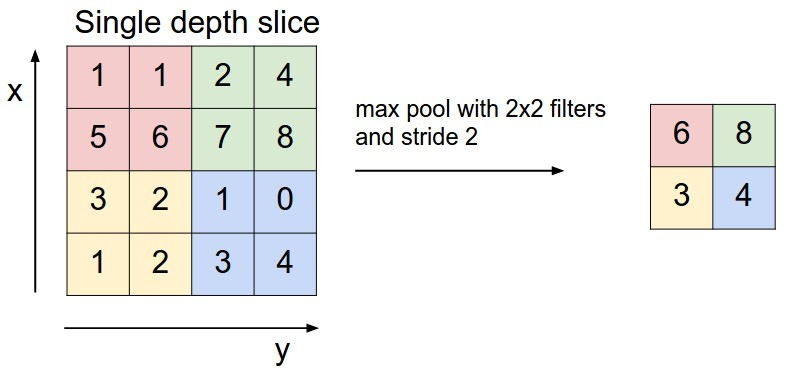
\includegraphics[width=0.8\textwidth]{\path/maxpool.jpeg} 
 \caption{Max pooling: the output image will have 1/4 of the input pixels.}
 \label{fig:maxpool}
\end{figure}

Through the network it is possible to gradually have a higher number of feature maps and therefore the richness of the representation of the features; and a decrease in the input resolution. These factors combined together give a strong degree of invariance to the geometric transformations of the input.

\subsection{Fully connected layer (FC)}
%% mention that now the convolution is used%% 

In the fully connected layer, all output matrices from convolution layers are flattened and given as a vector input to a fully connected neural network that will act as a classifier. The calculations in this final part are no more than matrix-multiplications plus a bias. By stacking three or more of them together we will obtain what is known as a \emph{multi-layer percepetron}.  

\\In figure \ref{fig:cnn3}, a CNN can be observed in the "act" of classifying a car image. The network filters are displayed during all the processing levels of the input, and then they terminate in a fully connected layer that outputs a probability. This probability is then translated into a score, from which the winning class is chosen.

\begin{figure}[h!]
 \centering
 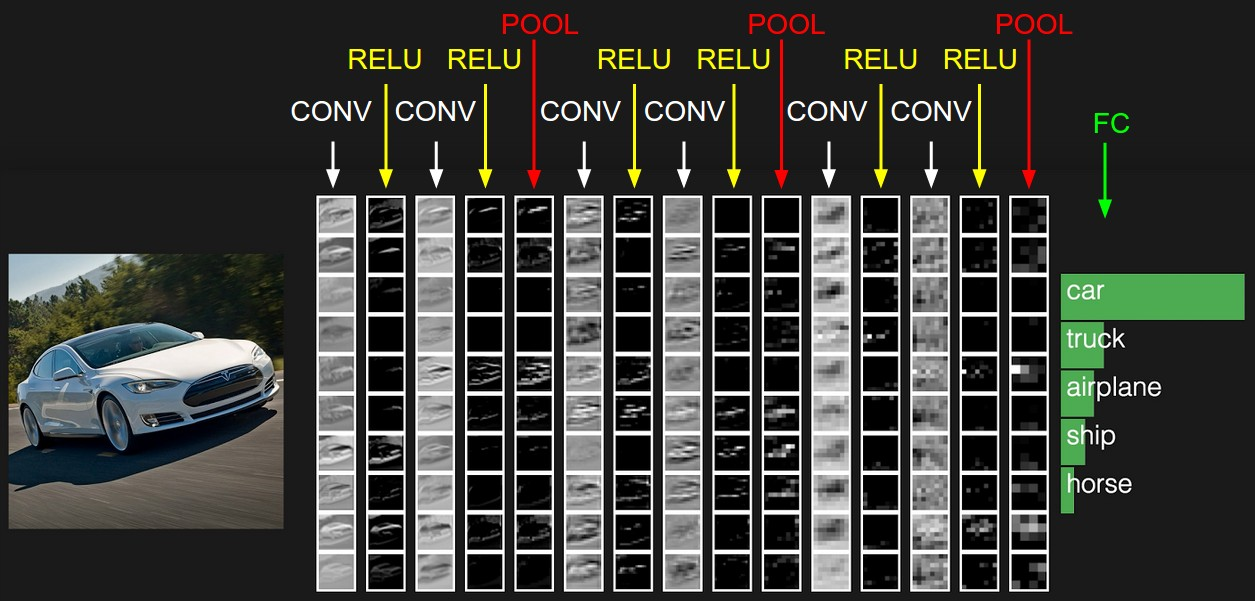
\includegraphics[width=1.0\textwidth]{\path/convnet.jpeg} 
 \caption{Typical CNN in a classification task; the winning class is the one with the highest probability, indicated at the end}
 \label{fig:cnn3}
\end{figure}

\subsubsection{Conversion of FC layers}
It has been noted recently that, except for the mode of connection, these neurons are functionally identical to those of convolution layers (both compute matrix multiplications). Thus, FC layers can be replaced with convolution layers that have a receptive field equal to the resolution of the images of the input \parencite{WCS231layer}. 

This conversion has two main advantages: 
\begin{itemize}
    \item \emph{efficiency}: all deep learning frameworks implements significant optimizations for the convolution operation, since convolutions are very commonly used. That could not be the case for less frequently used operations like matrix multiplications.
    
    \item \emph{input dimensions}: $[1 \times 1]$ convolutions enable to use image of different dimensions during testing. In fact, the convolution operation will slide on the whole image, one pixel at a time, which is impossible to do with FC layers. Therefore, in case the input image is bigger than those expected, the output of the network would be of size $O_w,O_h,M$ (instead of a simple $(1,1,M)$). Thus, the output will contain a map of probabilities with spatial references. This trick has been particularly useful in CNNs for object detection such as R-CNN and its successors \parencite{rcnn}. 
\end{itemize}



In Figure \ref{fig:cnn4} the complete architecture of a CNN is portrayed. It's noticeable how the resolution of the image is reduced to each pooling layer (also called subsampling) and how each pixel of the feature maps derives from the receptive field on the set of all the feature maps of the previous level. 


\begin{figure}[h!]
 \centering
 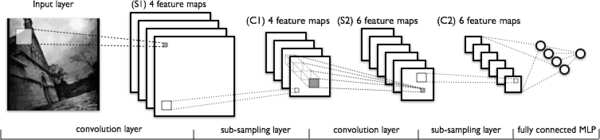
\includegraphics[width=1.0\textwidth]{\path/cnn-architecture.png} 
 \caption{Architecture of a CNN}
 \label{fig:cnn4}
\end{figure}




\paragraph{Summary} \newline 
Convnets expose a plethora of unique characteristics that made them the state of the art for computer vision. A quick recap of CNNs key points follows:

\begin{itemize}
    \item \emph{pipeline architecture}: in the general case CNNs are a sequence of CONV-RELU-(POOL) stacked together with a final linear classifier; 
    
    \item \emph{parameter sharing}: in order to reduce the otherwise huge number of parameters, each neuron from the same feature map share the same set of weights; 
    
    \item \emph{local connectivity}: each neuron is connected only to a small patch of the image; the size of this image is called \emph{receptive field}; 

    
    \item \emph{feature extraction}: lining up convolutional layers plus non-linear units enable CNNs to capture more abstract feature at every stage, building up a semantic understanding of the image; 
        
    \item  \emph{translation-invariance}: thanks to parameter sharing and local connectivity features are captured even if they are translated (in the input images); 
    
\end{itemize}

%--------------------------------------------------------------------
%	SECTION 3
%--------------------------------------------------------------------
\newpage
\section{CNN design}
In order to tackle a wide range of challenges, CNNs have become more and more complex in recent years. CNN comprise an enourmous design space, with numerous options for microarchitectures (see \ref{subsec:arch}), solvers and all the different hyperparameters; according to \parencite{cnn-design}, a small region of the CNN design space contains 30 billion different CNN architectures. Hence, it must not be surprising that the research community has been continuously discovering patterns that leads to more powerful models. 

Some of these significant milestones are introduced in this section. 

\subsection{One by one convolution layer}
\label{subsec:onebyone}
One by one convolution was first introduced in the architecture of the popular \emph{"Network-In-Network"} \parencite{NIN}, whose goal was to going "deeper" with convolutions. As already mentioned, stacked convolutional layers build up a semantic understanding of the image. Over the years, many experiments have shown how, in general ,adding more layers lead to better results.

However, convolution operations are costly, expecially when computed on a high number of filters like in convolutional layers. The intuition behind NIN was that $[1 \times 1$ convolution acts as a trick to make the network deeper while also being cheap. In fact, 
the complexity in this scenario drops down to $O(ST)$, with $S$ and $T$ being the number of input and output maps respectively. 
\newline

In this regard, it is interesting to notice that one by one convolutions are used to perform \emph{dimensionality reduction}: if we set $T < S$, the number of output channels will be reduced while the image size and features will be preserved. 
\\
Thus, it also acts as a feature pooling technique across the channels i.e., it reduces the number of channels while enhancing the strongest features, just like spatial pooling does on image patches (spatial pooling will be introduced in more details in section \ref{subsec:pooling}).
\newline 


Practically, one by one convolutions are no more than regular matrix multiplications (like in fully-connected layers) that perform linear re-combinations of the input pixel and thus are fast. It must be noted though, that even if the spatial size of the kernel is $[1x1]$ these multiplications are not a simple point-wise scaling, because they perform a dot product on one pixel but over the whole depth of the input channels. 
\newline 

There is more to it than just a sum of features across channels, though. One by one convolutions act like \emph{"coordinate-dependent transformation in the filter space"} \parencite{NIN}. It is important to point out that while this transformation is strictly linear, it is most often followed by non-linear activation layers. Therefore, this transformation is learned through gradient descent during training while also being robust against over-fitting thanks to the reduced number of parameters. 
\newline 

Looking at it from a wider point of view, one by one convolution builds up a mini deep neural network whose output is fed into the rest of the network. Hence the name Network-In-Network. 
\newline

As it will be explained in chapter 4, one by one convolution are one of the fundamentals to perform CNN compression through tensor decomposition. In fact, in order to boast a significant factor of compression on ordinary CNN structures, some tensor decomposition techniques pair this design strategy with the intuition of separable kernels described in section \ref{subsec:severino}.

\subsection{Depth-wise convolution layer}
\label{subsec:depthwise}
Depthwise separable convolutions perform spatial convolution while keeping the channels separate and then follow with a depthwise $[1 \times 1]$ convolution. This convolution is often erroneously called just \emph{"separable"} which collides with the definition given in \ref{subsec:separable}. 
\\

Figure \ref{fig:depthwise} shows the structure of a depthwise convolution. 

Recalling the example in section \ref{subsec:cnn-complexity}, it gets evident how these layers give an important reduction factor over standard convolution. 

For a depthwise separable convolution, the 16 input channels are traversed with only 1 $3 \times 3$ kernel each, giving in output 16 feature maps instead of 32. Now, before any merge happens, these 16 feature maps are traversed with 32 $1 \times 1$ convolutions each and only then are added together. This results in 656 $(16\times3\times3 + 16\times32\times1\times1)$ parameters opposed to the 4608 $(16\times32\times3\times3)$ parameters from the example of section \ref{subsec:cnn-complexity}.  

Formally the computational cost of this type of convolution is: 
\begin{equation}
    S\cdot d \cdot d + S \cdot T 
\end{equation}

Another important parameter of this design is the so called \emph{depth multiplier} which sets the number of depthwise convolutional output channels per input map. 

The example above is a specific implementation of a depthwise separable convolution where the depth multiplier is 1. This is by far the most common setup for such layers and have been made popular by F.Chollet within the Xception network \parencite{Xception}. 
\newline 

The core hypothesis of his work is that the mapping of cross-channels correlations and spatial correlations in the feature maps of convolutional neural networks can be \emph{entirely decoupled}. 


Looking at the results, this hypothesis held true as Xception outperforms even the popular \emph{inception} modules, from which they took inspiration from.

As the author puts it in conclusions: 
\begin{quote}
    We expect depthwise separable convolutions to become a cornerstone of convolutional neural network architecture design in the future,  since they offer similar properties as Inception modules, yet are as easy to use as regular convolution layers. 
\end{quote}

This thesis takes this hypothesis further by also decoupling the spatial convolution into a vertical and an horizontal step. 

%%% questi vanno dopo %%% 
\subsection{CNN Microarchitecture}
\label{subsec:arch}
With the trend of designing very deep CNNs, it becomes cumbersome to manually select filter dimensions for each layer. To tackle this issue, various various higher level building blocks, or \emph{modules} have been proposed. These modules, comprised of multiple convolution layers with a specific fixed organization, are then combined with additional ad-hoc layers to form a complete network. Hence, CNN \emph{microarchitecture} is a term that refers specifically to the internal organization of these individual modules. 

To describe how these building blocks are combined together to form an end-to-end CNN it is used the term \emph{macro-architecture} instead. 


\subsubsection{Inception module}
One by one convolution, described in section \ref{subsec:onebyone}, was immediately applied with success in GoogLeNet, which was the winner of the ImageNet challenge in 2014\parencite{googlenet}. Its main contribution was the developement of the \emph{inception module}, depicted in figure \ref{fig:inception}

\begin{figure}[h!]
 \centering
 \includegraphics[width=1.0\textwidth]{\path/inception.png} 
 \caption{Inception module: the building block of GoogLeNet.}
 \label{fig:inception}
\end{figure}

This module address the issue of not knowing a priori which kind of layer is the best choice to extract the features. Therefore this module provides a solution not to have to decide at all. In fact, it combines four different layers together so to have a richer feature representation. 

Throughout experiments the authors found out that the model was able, in a sense, to choose on its own, i.e. some type of layers were more beneficial on a stage of the network with respect to another, thus showed richer feature maps. Additionally, this architecture allows the model to recover both local feature via smaller convolutions and more abstracted features with larger convolutions. 
\newline 

Although this was already a breakthrough on its own, perhaps the most important concept of the work was \emph{dimensionality reduction}. Taking a closer look at figure \ref{fig:inception}, it is easy to notice the presence of diverse $[1 \times 1]$ convolution layers. These layers help to keep the number of parameters reasonably low by performing dimensionality reduction as explained in section \ref{subsec:onebyone}. 

Therefore, GoogLeNet was able to extract many different representations of the input image while avoiding a parameter explosion. Afterwards, different updated version of the inception modules were proposed. \parencite{incpetion3} \parencite{inception4}.

\subsection{Residual block}
Residual blocks were made popular in 2015 as the building block of \emph{deep residual networks} called ResNet, from Microsoft Research Asia \parencite{resnet}. ResNet is a \emph{very} deep CNN,comprising of 152 layers in its original version, which imposed itself as state of the art in all ILVSRC competition categories: classification, detection and localization. 
\newline 

Residual blocks are based on the insight of \emph{residual learning} (figure \ref{fig:resnet}, that works as follows: 
\begin{enumerate}
    \item the input goes through a \texttt{conv-relu-conv} sequence, producing a certain output called $F(x)$; 
    
    \item the original input is added to the latter: $H(x) = F(x) + x $; 
    
    \item $F(x)$ is called the residual learning. 
\end{enumerate}

Residual learning changed the state of the art by suggesting some new ideas: 
\begin{enumerate}
    \item instead of throwing away the original input and use only the feature maps representations of it, residual block keep the original information throughout the whole network; 
    
    \item each block peform a kind of fine-tuning (see later) of the information learned by the previous layers, thus being easier to optimize; 
    
    \item residual learning helps training very deep models by addressing the  \emph{vanishing gradients} issue. 
    
\end{enumerate}


\subsection{Fire module}
The Fire module was recently proposed within the SqueezeNet model by Iandola et al. 2017 \parencite{squeezenet}, which reached AlexNet like\parencite{AlexNet} accuracy on ImageNet while being \emph{50X} smaller. 

The design principles followed by the authors constitutes an interesing insights to achieve high accuracy with low number of parameters.  

Strategy 1.Replace 3x3 filters with 1x1 filters.Given a budget of a certain number of convolutionfilters,  we will choose to make the majority of these filters 1x1,  since a 1x1 filter has 9X fewerparameters than a 3x3 filter.Strategy 2.Decrease the number of input channels to 3x3 filters.Consider a convolution layerthat is comprised entirely of 3x3 filters. The total quantity of parameters in this layer is (number ofinput channels) * (number of filters) * (3*3).  So, to maintain a small total number of parametersin a CNN, it is important not only to decrease the number of 3x3 filters (see Strategy 1 above), butalso to decrease the number ofinput channelsto the 3x3 filters.  We decrease the number of inputchannels to 3x3 filters usingsqueeze layers, which we describe in the next section.Strategy 3.Downsample late in the network so that convolution layers have large activationmaps.In a convolutional network, each convolution layer produces an output activation map witha spatial resolution that is at least 1x1 and often much larger than 1x1.  The height and width ofthese activation maps are controlled by: (1) the size of the input data (e.g. 256x256 images) and (2)3

These ideas led to the creation of the Fire module, illustrated in figure \ref{fig:fire}

\begin{figure}[h!]
 \centering
 \includegraphics[width=1.0\textwidth]{\path/inception.png} 
 \caption{Inception module: the building block of GoogLeNet.}
 \label{fig:inception}
\end{figure}


\subsubsection{MobileNets}
 In the lights of these results, MobileNets have been integrated as the standard mobile-ready networks in a recent update of the popular framework Tensorflow [CITE].



%--------------------------------------------------------------------
%	SECTION 4
%--------------------------------------------------------------------
\section{Deep Learning}
In this section the main concepts to actually train a CNN are introduced. It is also provided a quick recap on general machine learning; however, as an in-depth discussion of the former is out of the scope of this thesis, this is not to be considered an exhausting explanation. For further details, please see the references. 

\subsection{Machine learning quick recap}
%% qua si parla di supervised learning, di backprop e compagnia bella copiandolo dalla Milano 
\subsubsection{Supervised learning}


\subsubsection{Backprop}

%%%
\subsection{Data preprocessing}

\subsection{Normalization}

\subsubsection{Batch normalization}

%%% 
\subsection{Initial solutions}

\subsubsection{Xavier initialization}

%%% 
\subsection{Overfitting}

%% scrivere velocissimaemente un elenco di tecniche per ridurre overfit 

\subsection{Transfer learning}

\subsection{Fine-tuning}


%--------------------------------------------------------------------
%	SECTION 5
%--------------------------------------------------------------------
\section{Applications}The high efficiency, the peculiar, advantageous architecture together with the huge technological progress of the hardware, have made CNN the most promising system for visual tasks, with the most varied application areas such as: recognition and facial tagging (think about Facebook), intelligent image search (think of Google Photos), autonomous cars, smartphones, robots, drones, (video) games and more. CNNs have also had excellent results in natural language processing; in the discovery of drugs, since by predicting the interactions between certain molecules and proteins they have helped discover potential biomolecules for the treatment of Ebola \parencite{WCNN}, just to name a few others. Already 3 years ago, in an article published by the KTH \parencite{Overfeat} artificial vision department, the use of "OverFeat", a CNN trained for the 2013 ImageNet Challenge, was analyzed. The article remakrs how they used this CNN "off-the-shelf" that is to say, ready, and without further training it, testing it against other finely perfected state-of-the-art methods developed until then. As tests, they have chosen activities that are gradually getting further and further from the original task for which OverFeat has been trained and, they have verified that OverFeat outclasses the above mentioned methods on any dataset (see the article for details) despite having been trained only through ImageNet. The article closes with a sentence that I quote:
\begin{quote}
\emph{“Thus, it can be concluded that from now on, deep learning with CNN has to be considered as the primary candidate in essentially any visual recognition task.”}
\end{quote}\\
\subsection{Comparison with humans}In 2011, CNNs first beat the man by reaching a 0.56 \% error against 1.16 \% of humans on the recognition of road signs in the "German Traffic Sign competition run by IJCNN 2011" competition.\\\\Two years ago, in the annual ILSVRC competition, now considered by the community as the "Artificial Vision Olympics", Microsoft Research Asia presented ResNet \parencite{resnet}: a 152-layer CNN that lowered the classification error ( 1000 classes) to \emph{only 3.6\%}. The result is impressive, given that a human being more or less able to recognize all the classes has an error of about 5-10%, see \parencite{Wkarpa}. \\\\Another historically difficult task for artificial vision was the recognition of partially occluded, upside down or displaced seen from different angles. However, in 2015 a team from the Yahoo Labs managed to get a CNN \parencite{WMit} to learn this task. \\The last milestone in chronological order of the "Man vs. Machine" challenge is undoubtedly \textsc{AlphaGo}\parencite{WAlphaGo}. AlphaGo is the first program to succeed in beating a professional human player (Lee Sedol, 18 times world champion) to the ancient Chinese game of Go. Go is known to be computationally extremely complex: there are $10^{170}$ possible combinations of the chessboard, a higher number than the atoms in the known Universe.
It is therefore unsuitable with a "brute force" approach.\\AlphaGo is based on a combination of deep learning + tree search. In particular, it uses 3 CNN: 2 "policy network" to choose the most winning strategy and 1 "value network" as a heuristic function to evaluate the corretness of a hypothetical move. In addition, the output of these networks is combined with a "Monte Carlo Tree Search" to get a final answer on the next move to play. More details can be found on the exhaustive paper published by DeepMind \parencite{AlphaGo}.

These results are sufficient to understand the potential of convolutional neural networks.


